\chapter{Java Dialoge}
\renewcommand{\chaptertitle}{Java Dialoge}

\lehead[]{\normalfont\sffamily\hspace*{-2.00cm}\textcolor{white}{\colorbox{lightblue}{\makebox[1.60cm][r]{\thechapter}}}\hspace{0.17cm}\textcolor{lightblue}{\chaptertitle}}
\rohead[]{\textcolor{lightblue}{\chaptertitle}\normalfont\sffamily\hspace*{0.17cm}\textcolor{white}{\colorbox{lightblue}{\makebox[1.60cm][l]{\thechapter}}}\hspace{-2.00cm}}
%\chead[]{}
\rehead[]{\textcolor{lightblue}{AvHG, Inf, My}}
\lohead[]{\textcolor{lightblue}{AvHG, Inf, My}}

\lstset{style=myJava}


\section{Dialoge verwenden}

Einfache Standard-Dialoge kann man mit der Klasse \myClass{JOptionPane} aus dem
Package \myPackage{javax.swing} erzeugen. Um auf die Klasse zugreifen zu können,
muss man folgende \verb|import|-Anweisung oben in der Datei einfügen:

\begin{lstlisting}
import javax.swing.*;
\end{lstlisting}

Das Sternchen bedeutet, dass alle Klassen aus dem Package
\myPackage{javax.swing} verwendet werden können. Alternativ kann man auch
explizit die Klasse angeben, auf die man zugreifen möchte, also:

\begin{lstlisting}
import javax.swing.JOptionPane;
\end{lstlisting}

\begin{center}
\begin{minipage}{1.0\textwidth}
\begin{framed}
In Java gibt es zwei große Bibliotheken (d.h. Code-Sammlungen), die fertigen
Code bereit stellen: AWT und Swing. Jede Bibliothek enthält mehrere
Unterkomponenten, die sogenannten Packages. Die Klasse \myClass{JOptionPane}
gehört -- wie man am Package-Namen erkennen kann -- zur Swing-Bibliothek.
\end{framed}
\end{minipage}
\end{center}

\subsection{Nachricht ausgeben}

Mit der folgenden Methode kann man einen einfachen Dialog mit einem
\myPMI{OK}-Button erzeugen:

\begin{lstlisting}
public static void showMessageDialog(Component parentComponent, Object message)
\end{lstlisting}

\begin{minipage}{0.6\textwidth}
Als ersten Parameter muss man das Anwendungsfenster übergeben. Als zweiten
Parameter wird die Nachricht angegeben (normalerweise als String).

\vspace{5mm}

Beispiel:
\end{minipage}\hfill
\begin{minipage}{0.30\textwidth}
\centering
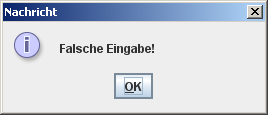
\includegraphics[width=1.0\textwidth]{./inf/SEKII/07_Java_Dialoge/MessageDialog.png}
\end{minipage}

\begin{lstlisting}
import javax.swing.*;                                      æ// Oben in der Datei 
 .
 .
 .
æJOptionPane.showMessageDialog(this, "Falsche Eingabe!");   æ// Irgendwo in einer 
                                                           // Methode
\end{lstlisting}

\begin{center}
\begin{minipage}{1.0\textwidth}
\begin{framed}
\verb|this| bezeichnet immer das aktuelle Objekt (so als wenn wir
Menschen „ich“ sagen). Wenn man im Anwendungsfenster
ist, bezeichnet \verb|this| das Anwendungsfenster.
\end{framed}
\end{minipage}
\end{center}

\begin{center}
\begin{minipage}{1.0\textwidth}
\begin{framed}
Methoden, die mit dem Schlüsselwort \verb|static| gekennzeichnet sind, kann man
benutzen, indem man einfach den Klassennamen davor setzt.
\end{framed}
\end{minipage}
\end{center}

\subsection{Eingabe-Dialog}

Mit folgender Methode kann man einen Dialog zum Einlesen eines Strings erzeugen:

\begin{lstlisting}
public static String showInputDialog(Object message)
\end{lstlisting}

Beispiel:

\begin{lstlisting}
String text = JOptionPane.showInputDialog("Gib eine Zahl ein:");
\end{lstlisting}

\begin{minipage}{0.30\textwidth}
\centering
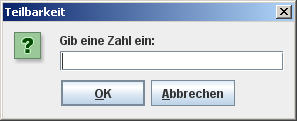
\includegraphics[width=1.0\textwidth]{./inf/SEKII/07_Java_Dialoge/InputDialog.png}
\end{minipage}\hfill
\begin{minipage}{0.6\textwidth}
Wenn der Benutzer den \myPMI{OK}-Button drückt, gibt die Methode
\verb|showInputDialog()| den eingegebenen Text als String zurück. Wenn der
\myPMI{Abbrechen}-Button gedrückt wird, ist der Rückgabewert \verb|null|
(Bedeutung: kein Objekt vorhanden).
\end{minipage}


\section{Nebenläufigkeit von Events in Swing}

In Programmen werden oft mehrere „Handlungsstränge“ (sogenannte \emph{Threads})
parallel ausgeführt. Ohne diese Nebenläufigkeit wäre es beispielsweise nicht
möglich die Benutzerschnittstelle (User-Interface oder auch kurz UI) für
Benutzerinteraktionen frei zu halten, während das Programm gleichzeitig eine
komplexe Berechnung ausführt oder auf etwas wartet.

\subsubsection{Swing ist nicht „Thread-Safe“}

Im Unterschied zu AWT ist Swing nicht Thread-Safe. Das bedeutet, dass der
Programmierer selbst dafür sorge tragen muss, dass nicht mehrere Threads
gleichzeitig versuchen auf ein Objekt zuzugreifen. Bis auf Weiteres reicht es
wenn ihr euch merkt, dass es im Zweifelsfall sinnvoll ist, Swing-Methoden nicht
direkt auszuführen, sondern diese an den sogenannten \emph{Event Dispatch Thread
(EDT)} zu übergeben:

\begin{lstlisting}
EventQueue.invokeLater(new Runnable() {
  public void run() {
    JOptionPane.showMessageDialog(null, "Game Over");
  }
});
\end{lstlisting}

Beachte dabei, dass als erstes Argument von \verb|showMessageDialog()| nicht
mehr this sondern \verb|null| benutzt werden muss!

Statt des in diesem Beispiel verwendeten \verb|showMessageDialog()| könnten es
auch beliebige andere Swing Methoden sein. Auch mehrere.

Zu beachten ist dabei, dass der Zeitpunkt der tatsächlichen Ausführung dieses
Befehls bzw. dieser Befehlsfolge nicht mehr unter der Kontrolle des
Programmierers liegt. Das folgendes funktioniert nicht:

\begin{lstlisting}
name = "Rumpelstilzchen";
EventQueue.invokeLater(new Runnable() {
  public void run() {
    name = JOptionPane.showInputDialog("Gib deinen Namen ein:");
  }
});
System.out.println("Hallo " + name + "!");
\end{lstlisting}

Richtig wäre es so:

\begin{lstlisting}
name = "Rumpelstilzchen";
EventQueue.invokeLater(new Runnable() {
  public void run() {
    name = JOptionPane.showInputDialog("Gib deinen Namen ein:");
    System.out.println("Hallo " + name + "!");
  }
});
\end{lstlisting}

Du findest dazu im Kursordner die Dateien \myFile{EDTfalsch.java} und
\myFile{EDTrichtig.java}.

Die Formulierung „im Zweifelsfall“ (oben) bedeutet, dass es durchaus auch ohne
den Umweg über den EDT funktionieren kann (und oft genug auch tut). Spätestens
dann, wenn Swing Elemente (Fenster und Dialoge) oder Teile davon nicht korrekt
dargestellt werden solltest du dich an den Hinweis auf den EDT besinnen und
diesen benutzen.